
% Template for Elsevier CRC journal article
% version 1.0 dated 13 October 2009

% This file (c) 2009 Elsevier Ltd.  Modifications may be freely made,
% provided the edited file is saved under a different name

% This file contains modifications for Procedia Computer Science

%%%%%%%%%%%%%%%%%%%%%%%%%%%%%%%%%%%%%%%%%%%%%%%%%%%%%%%%%%%%%%%%%%%%%%%%%%

%% This template uses the elsarticle.cls document class and the extension package ecrc.sty
%% For full documentation on usage of elsarticle.cls, consult the documentation "elsdoc.pdf"
%% Further resources available at http://www.elsevier.com/latex

%%%%%%%%%%%%%%%%%%%%%%%%%%%%%%%%%%%%%%%%%%%%%%%%%%%%%%%%%%%%%%%%%%%%%%%%%%

%% The '3p' and 'times' class options of elsarticle are used for Elsevier CRC
\documentclass[3p,times]{elsarticle}

%% The `ecrc' package must be called to make the CRC functionality available
\usepackage{ecrc}

%% The ecrc package defines commands needed for running heads and logos.
%% For running heads, you can set the journal name, the volume, the starting page and the authors

%% set the volume if you know. Otherwise `00'
\volume{00}

%% set the starting page if not 1
\firstpage{1}

%% Give the name of the journal
\journalname{Procedia Computer Science}

%% Give the author list to appear in the running head
%% Example \runauth{C.V. Radhakrishnan et al.}
\runauth{}

%% The choice of journal logo is determined by the \jid and \jnltitlelogo commands.
%% A user-supplied logo with the name <\jid>logo.pdf will be inserted if present.
%% e.g. if \jid{yspmi} the system will look for a file yspmilogo.pdf
%% Otherwise the content of \jnltitlelogo will be set between horizontal lines as a default logo

%% Give the abbreviation of the Journal.
\jid{procs}

%% Give a short journal name for the dummy logo (if needed)
\jnltitlelogo{Procedia Computer Science}

%% Hereafter the template follows `elsarticle'.
%% For more details see the existing template files elsarticle-template-harv.tex and elsarticle-template-num.tex.

%% Elsevier CRC generally uses a numbered reference style
%% For this, the conventions of elsarticle-template-num.tex should be followed (included below)
%% If using BibTeX, use the style file elsarticle-num.bst

%% End of ecrc-specific commands
%%%%%%%%%%%%%%%%%%%%%%%%%%%%%%%%%%%%%%%%%%%%%%%%%%%%%%%%%%%%%%%%%%%%%%%%%%

%% The amssymb package provides various useful mathematical symbols
\usepackage{amssymb}
%% The amsthm package provides extended theorem environments
%% \usepackage{amsthm}

%% The lineno packages adds line numbers. Start line numbering with
%% \begin{linenumbers}, end it with \end{linenumbers}. Or switch it on
%% for the whole article with \linenumbers after \end{frontmatter}.
%% \usepackage{lineno}

%% natbib.sty is loaded by default. However, natbib options can be
%% provided with \biboptions{...} command. Following options are
%% valid:

%%   round  -  round parentheses are used (default)
%%   square -  square brackets are used   [option]
%%   curly  -  curly braces are used      {option}
%%   angle  -  angle brackets are used    <option>
%%   semicolon  -  multiple citations separated by semi-colon
%%   colon  - same as semicolon, an earlier confusion
%%   comma  -  separated by comma
%%   numbers-  selects numerical citations
%%   super  -  numerical citations as superscripts
%%   sort   -  sorts multiple citations according to order in ref. list
%%   sort&compress   -  like sort, but also compresses numerical citations
%%   compress - compresses without sorting
%%
%% \biboptions{comma,round}

% \biboptions{}

% if you have landscape tables
\usepackage[figuresright]{rotating}

% put your own definitions here:
%   \newcommand{\cZ}{\cal{Z}}
%   \newtheorem{def}{Definition}[section]
%   ...

% add words to TeX's hyphenation exception list
%\hyphenation{author another created financial paper re-commend-ed Post-Script}

\providecommand{\e}[1]{\ensuremath{\times 10^{#1}}}
\usepackage[normalem]{ulem}
\usepackage{algorithmic}
% declarations for front matter

\begin{document}

\begin{frontmatter}

%% Title, authors and addresses

%% use the tnoteref command within \title for footnotes;
%% use the tnotetext command for the associated footnote;
%% use the fnref command within \author or \address for footnotes;
%% use the fntext command for the associated footnote;
%% use the corref command within \author for corresponding author footnotes;
%% use the cortext command for the associated footnote;
%% use the ead command for the email address,
%% and the form \ead[url] for the home page:
%%
%% \title{Title\tnoteref{label1}}
%% \tnotetext[label1]{}
%% \author{Name\corref{cor1}\fnref{label2}}
%% \ead{email address}
%% \ead[url]{home page}
%% \fntext[label2]{}
%% \cortext[cor1]{}
%% \address{Address\fnref{label3}}
%% \fntext[label3]{}

\dochead{International Conference on Computational Science, ICCS 2012}
%% Use \dochead if there is an article header, e.g. \dochead{Short communication}

\title{Towards speed up search of maximal unique matches in multicore architectures}

%% use optional labels to link authors explicitly to addresses:
%% \author[label1,label2]{<author name>}
%% \address[label1]{<address>}
%% \address[label2]{<address>}

\author{}

\address{}

\begin{abstract}
  Maximal Unique Matches are common substrings that are found between a reference and a query sequence. They are exact, unique and maximal; that is, they cannot be extended in left or right direction without incurring a mismatch. The computation of MUMs in large sequences is a heavy and repetitive task because the genomes are closely related, so there is a fair chance of parallelize and execute this search in multicore architectures. This research resembles a first novel approach to find MUMs in genomic sequences in parallel way. The reference genome is indexed by using a suffix tree in main memory and then the parallelized algorithm finds the MUMs against a query genome which is readed by several threads. This approach is based on MUMmer, a genome alignment tool, which is able to find Maximal Unique Matches (MUMs). 
\end{abstract}

\begin{keyword}
%% keywords here, in the form: keyword \sep keyword

%% PACS codes here, in the form: \PACS code \sep code

%% MSC codes here, in the form: \MSC code \sep code
%% or \MSC[2008] code \sep code (2000 is the default)

\end{keyword}

\end{frontmatter}

%%
%% Start line numbering here if you want
%%
% \linenumbers

%% main text
\section{Problem}
\label{}
The problem of searching maximal unique matching for a minimum lengthbetween a reference
string and a query string has been
identified in several applications, one of them is MUMmer. Altough
MUMmer's algorithm can perform searches of maximal unique matches (MUMs)
the use of resources are not well used:
\begin{itemize}
  \item High use of main memory to store the reference string.
  \item A null use of multicore architectures.
\end{itemize}
If the length of reference and query are very huge, the amount of operations to perform
in the search of MUMs increases, see table \ref{tbl:operations}.
\begin{table}[ h!]
  \begin{small}
    \begin{center}
      \begin{tabular}{lllll}
        Data structure & L [bp\footnote{Base pair, basic measure unit of nucleotides for a DNA sequence.}] & Search  & Search [s] & Memory\\
        & & operations & & usage [MB]\\
        \hline
        Suffix tree & 20 & 9,87\e{18}  & 169189,4 & 48665,12\\
        \hline
      \end{tabular}
    \end{center}
  \end{small}
  \caption{Search of Maximal Unique Matches between a reference sequence (2960,21Mbp) and query sequence (2716,96Mbp)}
  \label{tbl:operations}
\end{table}
The use of parallelism could help reduce the execution time for the search of maximal unique matches. One approach of
parallelism is to take advantage of multicore architectures nowadays.\\
This problem has a time complexity of $O(m+k)$ where $m$ is the length of the query sequence and $k$ is the number of 
maximal unique matches of some minimum length. This problem is a very high intensive computing task, for every substring
in the query sequence the search for a maximum unique match has to be performed.\\
\section{The MUM: an heuristic approach}
\subsection{Definition MUM}
Although a pair of conserved genes rarely contain the same entire sequence, they share a lot of short common substrings and some of them are indeed unique to this pair of genes. For example the following two sequences, R and Q:\\
\begin{center}
    R=\underline{ac} ga \underline{ctc} a \underline{gctac} t \underline{ggtcagctatt} \underline{acttaccgc}\$\\
      Q=\underline{ac} tt \underline{ctc} t \underline{gctac} \underline{ggtcagctatt} c \underline{acttaccgc}\$\\
    \end{center}
    It is clear that sequences R and Q have many common substrings, they are:
    \begin{itemize}
      \item ac
      \item ctc
      \item gctac
      \item ggtcagctatt
      \item acttaccgc
    \end{itemize}
Among those five common substrings, ac is the only substring that is not unique. It occurs more than once in both sequences. You can also observe that actually a, c, t, and g are common substrings of R and Q. However, they are not maximal, i.e. they are contained in at least one longer common substrings. We are only interested in those that are of maximal length.\\
Our aim is to search for all these short common substrings. Given genomes R and Q, we need to find all common substrings which are unique and of maximal length. Each of such common substrings is known as Maximum Unique Match (MUM). For almost every conserved gene pairs, there exist at least one MUM which is unique to them.\\
For example, assuming d = 3, sequences R and Q in the previous example has four MUMs: ctc, gctac, ggtcagctatt, acttaccgc. Substring ac is not an MUM because its length is smaller than the value of d and it is not unique to both sequences.
\begin{center}
    R=\xout{ac} ga \sout{ctc} a \uwave{gctac} t \uuline{ggtcagctatt} \uline{acttaccgc}\$\\
      Q=\xout{ac} tt \sout{ctc} t \uwave{gctac} \uuline{ggtcagctatt} c \uline{acttaccgc}\$\\
    \end{center}
The concept of MUM is important in whole genome alignment because a significantly long MUM is very likely to be part of the global alignment.
\subsubsection{Finding MUMs in a suffix tree} 
The key idea in this method is to build a suffix tree for genome R, a data structure which allows finding, extremely efficiently, all distinct subsequences in a given sequence.\\
  By construction, the location in the suffix tree represents a 
  substring of the subject sequence which maximaly matches a prefix of
  \texttt{querysuffix}. Thus it is only necessary to verify that,
  the substring of the subject sequence is long enough, that it
  is unique in the subject sequence and that the match
  is also left maximal. This is done as follows:
  
  \begin{enumerate}
  \item
  does \texttt{loc} represent a substring of length at least 
  \texttt{minmatchlength}?
  \item
  does \texttt{loc} correspond to a leaf edge? Then then the string 
  represented by the location is unique in the subject sequence.
  \item
  is the substring left maximal? This is true if one of the following
  conditions hold:
  \begin{itemize}
  \item
  the suffix of the query currently considered is the first suffix, or 
  \item
  the string represented by \texttt{loc} is a prefix of the subject string,
  or
  \item
  the characters immediately to the left of the matching strings
  in the subject sequence and the query sequence are different
  \end{itemize}
  \end{enumerate}
  If all conditions 1-3 are true, then a function 
  \texttt{processmumcandidate} is called. It takes the necessary 
  information about the MUM-candidate as its arguments. 
\subsubsection{Complexity analysis} 
\begin{itemize}
  \item \textbf{Step 1:} Building a suffix tree can be done in $O(n)$ time using McGreight's algorithm ~\cite{McCreight:1976:SST:321941.321946}.
  \item \textbf{Step 2:} Marking internal nodes takes $O(n)$ time. 
  \item \textbf{Step 3:} Comparing R[i-1] and Q[i-1] for each marked nodes takes $O(n+m)$ time as the number of marked nodes is at most $n+m-2$. By the same reasoning, traversing all internal nodes to extracting MUMs also takes $(n+m)$ time.
  \item In total,this algorithm takes $O(n+m)$ time to find all MUMs of the input sequences.
  \item The space complexity of this method is $O\left(n\log n\right)$ bits as we need to store the suffix tree of the input sequence.
\end{itemize}
Based on some experiments, it is found that MUMs can cover 100\% of the known conserved gene pairs. Moreover, finding all MUMs can be done in linear time.
\section{Parallelism technique}
%General-purpose, commodity CPUs currently have SIMD (Single Instruction Multiple Data) functional units and corresponding SIMD instructions. This kind of CPUs allow to be used in several ways of parallel techniques, such as data-level parallelism. \\
%In addition to using SIMD technology, the availability of HPC clusters makes possible to execute the same task with a different kind of data.\\
The sequential version of the MUMmer's algorithm trades extra computation for memory and high computation time when executed in a single machine. \\
Previously the algorithm for sequence alignment was described in detail. Now our own proposal of a parallelization of WGA with MUMmer is explained, Xipe Totec. There are two resources to improve in this algorithm:
\begin{itemize}
\item Memory usage.
\item Running time.
\end{itemize}
%The former was generally improved because it allows to be executed in environments where there is no restriction memory. 
To improve the performance of the algorithm a data-level parallelism technique is deployed in advance to genome alignment.\\
Our technique is divided in three phases following:
\begin{enumerate}
\item Splitting genome data according to the number of available cores.
\item Parallel execution of as many instances of mummer as available cores.
\item Get the list of MUMs from the whole set of MEMs\footnote{Maximal Exact Match} found in the previous phase.
\end{enumerate}
The following Figure \ref{algorithm} shows the process of our data-level parallelism technique.
\begin{figure}[htb] 
\begin{center} 
  %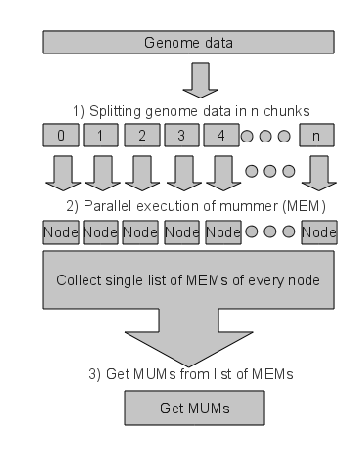
\epsfig{file=algorithm.eps,width=4.5cm,height=4cm} 
\end{center} 
\caption{Data-level parallelism technique for whole genome alignment.} 
\label{algorithm} 
\end{figure} 
The division of genome data was used using the paradigm of data-level parallelism which consists of a generation of chunks of a sequence with a fixed size and a fixed overlap. One issue arises when a genome is splitted because of the heuristic used in the algorithm is affected. So that, a longer sequence is more likely to have a better finding of MUMs while a smaller one can produce MUMs which are not effective MUMS.\\
Another consideration was the genome structure, because a genome is build from a finite alphabet $\Sigma=\{a,g,c,t,n\}$ but according to the MUMmer's algorithm each alignment is made using only the nucleotide base pairs, this means that letter "n" in a biological way can mean anything: (a,g,c,t). A complex structure of a genome can have a huge impact of our data level parallelism.\\
%The main idea in MUMmer is its heuristic, Maximal Unique Match (MUM), based on this concept it is possible to cover a huge region of a genome when reference and query genomes are very closely related. However 
To get a MUM, it requires an important feature its uniqueness. 
%We had to face with concept while we evaluated different ways to implement the data-level parallelism. 
Uniqueness can only be found when a whole genome is checked.
%if some part of it is only evaluated we could miss the rest of the genome. 
In other words, after finding MUMs within a chunk it is not possible to determine if the MUM found is or not a "unique" MUM, globally in the genome,  because these MUMs are unique only in the chunk that has been read, the rest of the genome it is not known.\\
One solution to solve this problem is to drop the MUMmer's heuristic in order to be able to find the correct MUMs when we apply our data-level parallelism. The new approach is to find a Maximal Exact Match (MEM), a MEM allows to drop the uniqueness of a match but with a high computational cost: a brute-force approach.\\
%A MEM as shown in Figure \ref{mem} has the advantage of getting the true MUMs regardless a division of genome data. In Figure \ref{mem} R stands for reference genome and Q stands for query genome, this example shows that blue and red matches have exact matches but turn out not to be unique, then not a valid MUM; a true MUM is the green match.\\
Nevertheless, the major problem with the use of MEM is that the number of occurrences increases exponentially when \emph{shorter MEM} are used. Moreover, the high ratio of MEMs requires to save them in some place, memory or disk, that means a heavy use of resources in both CPU and Memory. This drawback is the main disadvantage because the hits of MEMs are increasing with the size of the genome. A new phase has to be designed to reduce the use of resources when a short MEM is searched.
%\begin{figure}[htb] 
%\begin{center} 
%  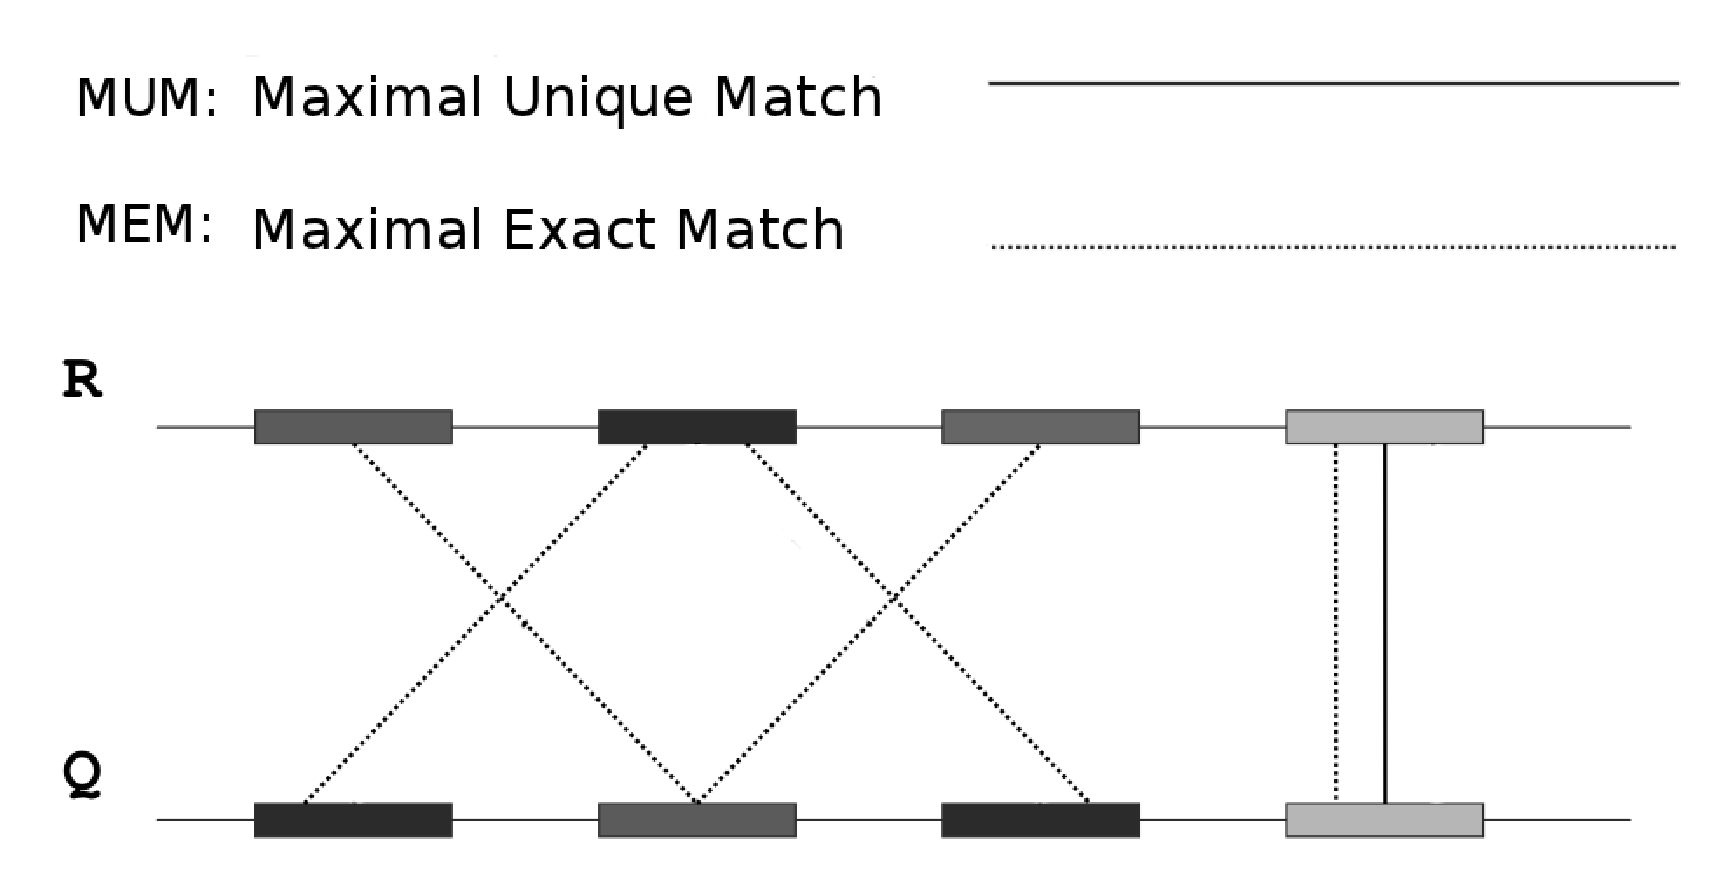
\epsfig{file=mem.eps,width=6cm, height=3cm} 
%\end{center} 
%\caption{Types of matches}
%\label{mem} 
%\end{figure} 
\section{Implementation} 
\label{implementation}
%When there is only one query sequence, one can try to split the query sequence and assign each part to a processor. This part covers in detail every aspect of Xipe Totec.
This section explains in detail how our proposal is implemented and the modifications in order to be executed in MUMmer. The following diagram, see Figure \ref{xipe-totec}, shows the add-ons of our approach, one is executed before MUMmer and the another after MUMmer.
\begin{figure}[htb]  
 \begin{center} 
   % 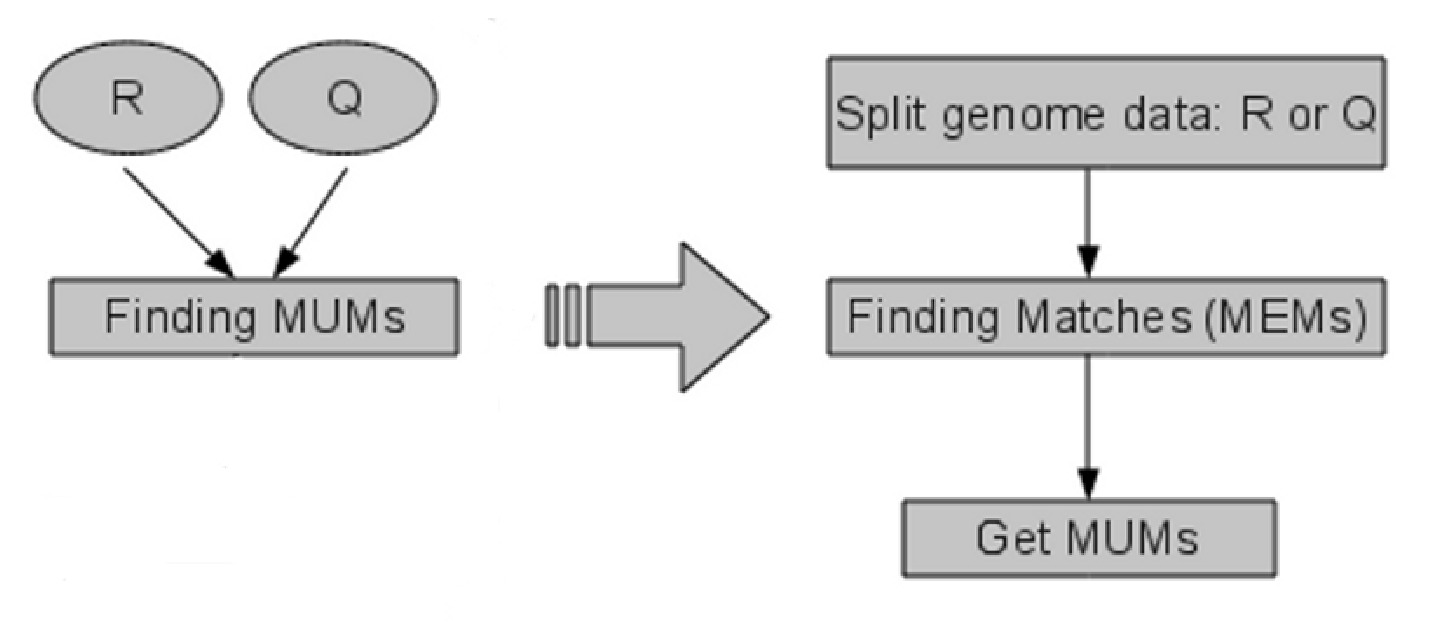
\epsfig{file=xipe-totec1.eps,width=7.5cm} 
 \end{center}
 \caption{Xipe Totec: proposal for parallelization of whole genome alignment} 
 \label{xipe-totec} 
\end{figure}
The following sections explain how the split of genome data, search of MEMs and get MUMs are carried out in our proposal.
\subsection{Split genome data} 
As it was previously explained, the approach is to use a fixed size division of genome data in as many chunks as  many available cores. Xipe Totec needs to know how many cores will be used in order to divide the genome data.\\
One key aspect of Xipe Totec is the way to split a genome. To align a genome requires a reference genome so that, there are two ways of using Xipe Totec:
\begin{itemize}
\item Splitting reference genome.
\item Splitting query genome.
\end{itemize}
Both of them can reduce the computation time or memory usage.\\
To split genome data a perl script was coded to do this task, the script requires the following arguments:
\begin{itemize}
\item Genome data to be splitted.
\item Number of chunks.
\item Overlap size.
\item Location to save the genome data.
\end{itemize}
\subsection{Finding MEMs}
This phase requires the mummer program, one of the several small programs in the MUMmer suite. mummer has several options.
In order to get a correct alignment, our proposal requires to compute MEMs instead of MUMs, so that mummer is executed with:
\begin{itemize}
  \item -n: to match only nucleotides.
  \item -maxmatch: option to get MEMs.
  \item -l \emph{length}: to find MEMs of a some minimum length.
\end{itemize}
List of MEMs is saved to a file which has the following format:
\begin{verbatim}
>Information about the sequence
Position_in_R Position_in_Q Length_of_MEM
\end{verbatim}
This list has to be joined with the output of every chunk computed and then the whole list is  manipulated in the following phase, \ref{getting}.
\subsection{Getting MUMs}
\label{getting}
This is the most important phase in our approach because it outputs the final list of MUMs those that are the same to the serial execution of mummer.\\
This phase needs the list of MEMs to process them and find those matches that are unique. The following diagram shows the basic idea behind this phase, see Figure \ref{xt}.
\begin{figure}[htb]  
 \begin{center} 
   %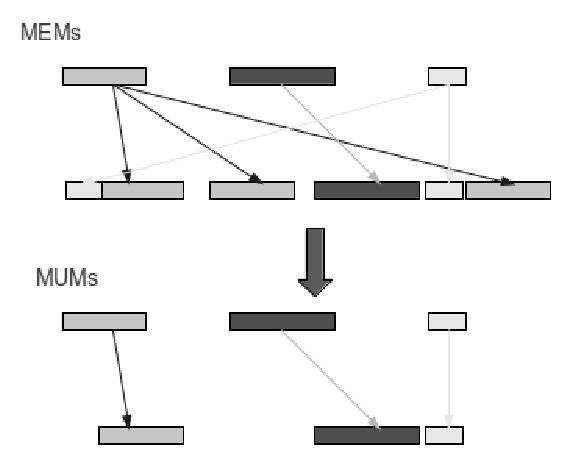
\epsfig{file=xt.eps,width=5cm, height=2cm} 
 \end{center} 
 \caption{Xipe Totec: Finding the real MUMs} 
   \label{xt} 
\end{figure}
To get the MUMs we filter those MEMs that are unique in the list and order them using a modified version of LIS\footnote{Longest Increasing Subsequence} algorithm.
The algorithm is shown below:
\begin{algorithmic}
\STATE{Input: List of MEMs: Position in R, position in Q, length of MEM}
\STATE{Sort MEMs by increasing position and decreasing length in R}
\FOR{$i:=0$ to $n$ in Total\_MEMs}
\IF{MEM[$i$] is not unique}
\STATE{Sort this subset by increasing position in Q and pick up the first MEM and drop the rest}
\ELSE {}
\STATE{MEM[$i$] is a MUM}
\ENDIF
\ENDFOR
\STATE{Sort MEMs by increasing position and decreasing length in Q}
\FOR{$i:=0$ to $n$ in Total\_MEMs}
\IF{MEM[$i$] is not unique}
\STATE{Sort this subset by increasing position in R and pick up the first MEM and drop the rest}
\ELSE {}
\STATE{MEM[$i$] is a MUM}
\ENDIF
\ENDFOR
\end{algorithmic}
The output of this algorithm gives the MUMs.
\section{Experiments and results}
To verify that our approach, Xipe Totec, can align a whole genome a set of tests were analyzed. These tests were carried out in a cluster with the following features:
\begin{itemize}
\item Hardware: 
\begin{itemize}
\item Processor Dual-Core Intel(R) Xeon(R) CPU 5160 @ 3.00GHz 4MB L2 (2x2)
\item Number of processors: 2
\item RAM: 12 GB Fully Buffered DIMM 667 MHz
\end{itemize}
\item  Software:
\begin{itemize}
\item Linux Kernel 2.6.16.46-0.12-smp x86\_64 GNU/Linux
\item gcc 4.3.2
\item MUMmer 3.22
\item Perl 5.8.8
\end{itemize}
\end{itemize}
%% The Appendices part is started with the command \appendix;
%% appendix sections are then done as normal sections
%% \appendix

%% \section{}
%% \label{}

%% References
%%
%% Following citation commands can be used in the body text:
%% Usage of \cite is as follows:
%%   \cite{key}         ==>>  [#]
%%   \cite[chap. 2]{key} ==>> [#, chap. 2]
%%

%% References with BibTeX database:
\section*{References}
\bibliographystyle{elsarticle-num}
\bibliography{<your-bib-database>}

%% Authors are advised to use a BibTeX database file for their reference list.
%% The provided style file elsarticle-num.bst formats references in the required Procedia style

%% For references without a BibTeX database:

% \begin{thebibliography}{00}

%% \bibitem must have the following form:
%%   \bibitem{key}...
%%

% \bibitem{}

% \end{thebibliography}

\end{document}

%%
%% End of file `procs-template.tex'. 
